\documentclass{beamer}

\input{../../spec_files/course_preamble.tex}
\subtitle{Foundations of Neuro-Symbolic AI}
\date{Summer Term 2026}
\author[FONS]{Alex Goessmann}
\institute[]{
    University of Applied Science Würzburg-Schweinfurt
%    Weierstrass Institute for Applied Analysis and Stochastic
}

%\newcommand{\techwstitle}{
%\small
%%Workshop \\
%Logik für Erklärbare KI:
%Technische Einführung in das ENEXA Projekt}
%\newcommand{\smalltechwstitle}{ENEXA Workshop}

%\newcommand{\techwsdate}{15.+16. July, 2024}

%\newcommand{\techwsauthors}{
%Alex Goessmann
%}

%\newcommand{\techwsinclude}{
%	\usepackage{../../spec/beamercolorthemeclaw}
%	\usepackage{/Users/alexgoessmann/Documents/ENEXA/latex_macros/beamer_template/beamerfontthemeclaw}
%	\usepackage{/Users/alexgoessmann/Documents/ENEXA/latex_macros/beamer_template/beamerinnerthemeclaw}
%	\usepackage{/Users/alexgoessmann/Documents/ENEXA/latex_macros/beamer_template/beamerouterthemeclaw}
%
%	\input{/Users/alexgoessmann/Documents/ENEXA/latex_macros/packages.tex}
%	\input{/Users/alexgoessmann/Documents/ENEXA/latex_macros/macros.tex}
%	\input{/Users/alexgoessmann/Documents/ENEXA/latex_macros/macros_tc.tex}
%	\input{/Users/alexgoessmann/Documents/ENEXA/latex_macros/tikz_blocks.tex}
%
%	\subtitle{\techwstitle}
%	\date[\techwsdate]{\techwsdate}
%	\author[\smalltechwstitle]{\techwsauthors}
%	\institute[]{\eupic}
%}

\newcommand{\techwschapterone}{I-Tensors}
\newcommand{\techwschaptertwo}{II-Probabilities}
\newcommand{\techwschapterthree}{III-Logics}
\newcommand{\techwschapterfour}{IV-Applications}

\newcommand{\eupic}{
\begin{center}
	%\includegraphics[width=4cm]{/Users/alexgoessmann/Documents/ENEXA/latex_macros/images/fundedEU.png}
\end{center}
}

\newcommand{\enexadateveublock}{
\begin{center}\begin{tikzpicture}
  	%\node [anchor=center] at (0,0) {\includegraphics[width = 1.5cm]{/Users/alexgoessmann/Documents/ENEXA/latex_macros/images/DATEV.png}};
	%\node [anchor=center] at (2.5,0.5) {\includegraphics[width = 3.5cm]{/Users/alexgoessmann/Documents/ENEXA/latex_macros/images/enexa.png}};
	%\node [anchor=center] at (2.55,-0.5) {\includegraphics[width = 3cm]{/Users/alexgoessmann/Documents/ENEXA/latex_macros/images/fundedEU.png}};
\end{tikzpicture}\end{center}
}


%% OLD
\newcommand{\aselectionvariable}{L}
\newcommand{\vselectionvariable}{L}
\newcommand{\fselectionvariable}{L}
\newcommand{\cselectionvariable}{L}
\newcommand{\individualorder}{n}
\newcommand{\variableof}[1]{\indvariableof{#1}}
\newcommand{\sindex}{s}
\newcommand{\pindex}{p}
\newcommand{\oindex}{o}
\newcommand{\exquery}{q}
%\newcommand{\datapointof}[1]{x^{#1}}
\newcommand{\atomicqueryof}[1]{g_{#1}}
\newcommand{\facsystem}{\shortcatvariables}
\newcommand{\margprobof}[1]{\probat{#1}}
\newcommand{\mlnprobabilityof}[1]{\expdistof{#1}}
%\newcommand{\oldenexadateveublock}{
%	\begin{center}
%	\begin{minipage}{0.2\textwidth}
%		\begin{center}
%			\includegraphics[width = 2.5cm]{images/DATEV.png}
%		\end{center}
%	\end{minipage}
%	\begin{minipage}{0.55\textwidth}
%		\begin{center}
%			\includegraphics[width=5.5cm]{images/enexa.png} \\
%			\includegraphics[width=5.5cm]{images/fundedEU.png} \\
%		\end{center}
%	\end{minipage}
%	\end{center}
%}

\title[Trends in AI]{
	\techwschapterone \\
	{\huge Trends in AI and the ENEXA Project}
}

\begin{document}



{\frame[plain]{\titlepage}}


\section{Motivation: Reasoning, its mechanization and computations}


\begin{frame}{How to approach Artificial Intelligence?}


\begin{block}{Learning: Inductive Reasoning}
	Use training data to identify models representing the knowledge about a system.
	%\begin{itemize}
		%\item Model represents \emph{knowledge} about the system
		%\item Inductive: Modelling assumptions and priors are important
	%\end{itemize}
\end{block}

\begin{center}
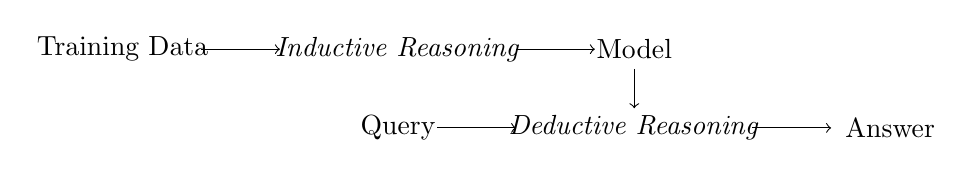
\begin{tikzpicture}
  	\node [anchor=center] at (0,0) {Training Data};
	\draw[->] (1,0) -- (2,0);
	 \node [anchor=center] at (3.5,0) {\emph{Inductive Reasoning}};
	 \draw[->] (5,0) -- (6,0);
  	\node [anchor=center] at (6.5,0) {Model};		
	 \draw[->] (6.5,-0.25) -- (6.5,-0.75);
	 \node [anchor=center] at (3.5,-1) {Query};
	 \draw[->] (4,-1) -- (5,-1);
	 \node [anchor=center] at (6.5,-1) {\emph{Deductive Reasoning}};
	 \draw[->] (8,-1) -- (9,-1);
	  \node [anchor=center] at (9.75,-1) {Answer};
\end{tikzpicture}
\end{center}

%Use the model of the system
%\begin{itemize}
%	\item Evidence (features) of a new datapoint
%	\item Inference given evidence
%\end{itemize}
\begin{block}{Inference: Deductive Reasoning}
	Retrieve specific parts of the knowledge based on a query containing evidence.
\end{block}

\end{frame}



\begin{frame}{How to mechanize Reasoning?}

\begin{block}{Modelling assumptions}
	\begin{itemize}
		\item \textbf{Ontological}: What properties does a system have? \\
			\hspace{0.5cm} $\rightarrow$ We assume \emph{fixed sets of categorical properties}.
		\item \textbf{Epistemological}: What can we tell about these properties? \\
			\hspace{0.5cm} $\rightarrow$ We associate \emph{possibilities or probabilities} with states.
	\end{itemize}
\end{block}
		
Two main frameworks differing in the \emph{empistemological} assumptions:
\begin{itemize}
	\item Logics (\emph{Possibilities}): The traditional mathematical model of intelligence. 
	\item Probability Theory (\emph{Probabilities}): Handling uncertainties about the systems state.
\end{itemize}
In both cases, we encode our knowledge in an arrangement of numbers: \emph{Tensors} with efficient representations by \emph{Tensor Networks}.

\end{frame}




\begin{frame}{A computational interface: \\
 Tensors in Artificial Intelligence}

On the \emph{software} side:
\begin{itemize}
	\item Parallel computing based on tensor algebra
	\item Standard ML libraries: TensorFlow, Pytorch
\end{itemize}

On the \emph{hardware} side:
\begin{itemize}
	\item Dedicated for graphic processing: Graphic Processing Units (GPUs)
	\item AI-dedicated hardware: Tensor Processing Units (TPUs)
\end{itemize}
\begin{center}
	\includegraphics[width=0.5\textwidth]{images/tensorflow.png}
	\includegraphics[width=0.2\textwidth]{images/nvidia-a100.jpeg}
	\includegraphics[width=0.3\textwidth]{images/google_tpu.png}
\end{center}
\end{frame}




\begin{frame}{Do Large Language Models (LLM) suffice for reasoning?}

Approach to
\begin{itemize}
	\item \emph{Inductive Reasoning}: LLMs are trained on massive amount of data and store knowledge in their weights
	\item \emph{Deductive Reasoning}: LLMs answer prompts to retrieve knowledge in a specific context
\end{itemize}

LLMs make use of tensors:
\begin{itemize}
	\item Organize computations in tensor contractions (layers of neural nets)
	\item Draw on AI-dedicated hardware for scaling
\end{itemize}

\begin{block}{Two major concerns about LLMs}
	Besides having astonishing knowledge representation capabilities, LLMs lack in
	\begin{itemize}
		\item \textbf{Explainability:} Problems with Halluzinations
		\item \textbf{Efficiency:} Massive power consumptions during reasoning
	\end{itemize}
\end{block}

\end{frame}





\begin{frame}{Outlook: The Neuro-Symbolic AI Initiative}

Neural Paradigm: Bringing \emph{efficiency}
\begin{itemize}
	\item Computations (gradients/inference) organized in layers (sets of neurons with tensor weights)
	\item Deep layers providing effective representation of data (task-dedicated neurons)
\end{itemize}

Symbolic AI: Bringing ante-hoc \emph{explainability}
\begin{itemize}
	\item Based on human interpretable logic
	\item Traditional approach to AI
\end{itemize}

\begin{block}{How to bring both paradigm together?}
	Design neural architectures representing symbolic reasoning.
\end{block}

\end{frame}








\section{The ENEXA project at DATEV}



\begin{frame}{The ENEXA project: \\ Efficient and Explainable Learning on Knowledge Graphs}
\centering
	\includegraphics[width=0.9\textwidth]{images/ENEXA_overview.png}
\end{frame}

\begin{frame}{Organizational Overview of ENEXA}
Scientific Methods:
\begin{itemize}
	\item Knowledge Extraction based on Large Language Models:\\ 
		\emph{University of Amsterdam (Prof. Paul Groth)}
	\item Knowledge Representation and Reasoning in Knowledge Graphs: \\
		\emph{University of Paderborn (Prof. Axel Ngonga)}
	\item Reasoning under Inconsistencies and Uncertainties: \\
		\emph{NCSR Demokritos Athens (Prof. Alexander Artikis)}
\end{itemize}

Targeted Use Cases:
\begin{itemize}
	\item Geospatial Intelligence: \emph{SatCen} (Madrid)
	\item Brand Communication: \emph{webLyzard} (Vienna)
	\item Business Software: \emph{DATEV} (Nuremberg)
\end{itemize}

%\begin{center}
%\includegraphics[width=8cm]{/Users/alexgoessmann/Documents/ENEXA/latex_macros/images/enexa.png}
%\end{center}

\end{frame}






\section{Further Trends}


\begin{frame}{ENEXA for Explainable AI}

ENEXA provides \textbf{intrinsic and ante-hoc} explainable models.
\begin{itemize}
	\item Logic as an interface between human and machine reasoning
	\item Humans can interpret and manipulate learned models
	\item Interpretations are globally valid, that is for all possible inputs to the model
	\item Guarantees on the behavior of the model can be derived
\end{itemize}

This is in contrast with typical \textbf{post-hoc} approaches to open black-box models at single datapoints.

\end{frame}



\begin{frame}{ENEXA for Causal AI}

Bayesian Networks are defined on directed graphs, which model causes and effects:
\begin{center}
	\includegraphics[width=5cm]{images/burglary.png}
\end{center}

In ENEXA we go one step beyond and represent cause and effect relationships in terms of probabilistic logics.

\begin{block}{Challenge}
	Since causality requires intervention with data or expert knowledge, how can we certify the causality of our models?
\end{block}



\end{frame}



\begin{frame}{Downsides of the rich architecture}

%	ENEXA methods have a rich mathematical structure, enabling tackling Explainable- Neuro-Symbolic and Causal AI

	\textbf{Expressivity:}
	\begin{itemize}
		\item Small sets of logical sentences have limited expressivity
		\item Model training and interpretation as an interactive process
	\end{itemize}
	\textbf{Efficiency:}
	\begin{itemize}
		\item Reasoning algorithms come with worst-case infeasibilities
		\item Tradeoff between exactness and efficiency
	\end{itemize}
	
	\begin{block}{Requirements for Use Cases}
		\begin{itemize}
			\item Small number of discrete random variables (when requiring exact reasoning)
			\item Larger numbers can only be handled with approximative algorithms
			\item Intuition about their logical interdependence for training and human interpretation
		\end{itemize}	
	\end{block}
\end{frame}




\end{document}







\begin{frame}{ENEXA at DATEV}


We 

	\begin{columns}
		\column{0.35 \linewidth}
		\begin{center}
			\textbf{Modelling} \\
			{Representation of accounting data as \\ 
			\emph{Knowledge Graphs}} \\
		%	Logical reasoning about \\ 
		%	\emph{connectivity}
		\end{center}
		\column{0.125 \linewidth}		
			\centering
			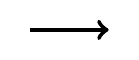
\begin{tikzpicture}
  				\draw[->, ultra thick] (0,0) -- (1,0);
			\end{tikzpicture}

		\column{0.475 \linewidth}
		\begin{center}
		\textbf{Reasoning} \\
			{Statistical Models }
			{Statistical dependencies of links} \\
			Probabilistic reasoning about \emph{samples}
			
		\end{center}
		
	\end{columns}

\end{frame}





\begin{frame}{Recommended Literature}

Introductory Textbooks on Logical and Probabilistic Reasoning:
\begin{itemize}
	\item \textbf{Russel, Norvig: Artificial Intelligence - A Modern Approach} (Fourth Edition), Pearson Education 2021 \\
		Parts III (Logics) and IV (Probability Theory)
	\item \textbf{Murphy: Machine Learning - A Probabilistic Perspective}, MIT 2012 \\
		Chapters 2-5, 20-24 (Probability Theory)
	\item \textbf{Antoniou et al: A Semantic Web Primer} (Third Edition), MIT 2012
\end{itemize}

Advanced Textbooks:
\begin{itemize}
	\item \textbf{Koller, Friedman: Probabilistic Graphical Models: Principles and Techniques}, MIT Press 2009
		%Representation and Reasoning with Bayesian and Markov Networks
	\item \textbf{Hackbusch: Tensor Spaces and Numerical Tensor Calculus} \\
		%Numerical foundations of Tensors
	\item \textbf{Brachman, Levesque: Knowledge Representation and Reasoning}, Morgan Kaufman 2004
\end{itemize}

\end{frame}














